\documentclass[10pt]{article}
\usepackage{adjustbox}
\usepackage{booktabs}
\usepackage{graphicx}
\usepackage{graphics}
%\usepackage{subcaption}
\usepackage{caption}
\usepackage{mathtools}
\usepackage{tikz,pgfplots}
\usepackage{subfig}
\usepackage{epsfig}
\usepackage{amsmath}
\usepackage{amssymb}
\usepackage[shortlabels]{enumitem}
\usetikzlibrary{angles,patterns,calc}
\usepackage{bbm}
\usepackage{float}
\usepackage{natbib}
\usepackage[sc]{mathpazo}
\usepackage[T1]{fontenc}
\usepackage{amsfonts}
\usepackage[onehalfspacing]{setspace}
\usepackage[margin=.75in, tmargin=0.71in, bmargin=0.71in]{geometry}
\usepackage{url}
\usepackage{appendix}
\usepackage{hyperref}
\usepackage{xcolor}
\usepackage{todonotes}
\usepackage{lscape}
\usepackage{comment}
\newcommand\der[2]{\frac{\partial{#1}}{\partial{#2}}}
\DeclareMathOperator*{\argmax}{arg\,max}
\DeclareMathOperator*{\argmin}{arg\,min}
\newtheorem{claim}{Claim}
\newtheorem{claimproof}{Proof of claim}[claim]

% stuff to put matlab code in 
\usepackage{listings}
\usepackage{color} %red, green, blue, yellow, cyan, magenta, black, white
\definecolor{mygreen}{RGB}{28,172,0} % color values Red, Green, Blue
\definecolor{mylilas}{RGB}{170,55,241}

% Shortcut greek
\def\a{\alpha}
\def\b{\beta}
\def\g{\gamma}
\def\D{\Delta}
\def\d{\delta}
\def\z{\zeta}
\def\k{\kappa}
\def\l{\lambda}
\def\n{\nu}
\def\r{\rho}
\def\s{\sigma}
\def\t{\tau}
\def\x{\xi}
\def\w{\omega}
\def\W{\Omega}

\usepackage[utf8]{inputenc}
\usepackage[english]{babel}
\usepackage{fancyhdr}
\fancypagestyle{firststyle}
{
\fancyhf{}
    \renewcommand{\headrulewidth}{0pt}
   \fancyfoot[C]{\footnotesize Page \thepage\ of \pageref{LastPage}}
}

\newcommand{\numpy}{{\tt numpy}}    % tt font for numpy

\usepackage[autostyle, english = american]{csquotes}
\MakeOuterQuote{"}

\topmargin -.5in
\textheight 9in
\oddsidemargin -.25in
\evensidemargin -.25in
\textwidth 7in

\newcommand{\question}[1]{ \begin{center} \noindent\colorbox{gray!10}{
\parbox{0.8\textwidth}{\vspace{0.125in} #1 \vspace{0.125in} } } \end{center} }

\floatplacement{table}{H}
\floatplacement{figure}{H}

\pgfplotsset{compat=1.17}

\begin{document}

    \thispagestyle{firststyle}

    \author{Isaac Liu, Nicol\'as Martorell \& Paul Opheim}
    \title{Principal Component Regression as a Solution to Measurement Error Bias} 
    \maketitle

    % code

    \lstset{language=Matlab,%
        %basicstyle=\color{red},
        breaklines=true,%
        morekeywords={matlab2tikz},
        keywordstyle=\color{blue},%
        morekeywords=[2]{1}, keywordstyle=[2]{\color{black}},
        identifierstyle=\color{black},%
        stringstyle=\color{mylilas},
        commentstyle=\color{mygreen},%
        showstringspaces=false,%without this there will be a symbol in the places where there is a space
        numbers=left,%
        numberstyle={\tiny \color{black}},% size of the numbers
        numbersep=9pt, % this defines how far the numbers are from the text
        emph=[1]{for,end,break},emphstyle=[1]\color{red}, %some words to emphasise
        %emph=[2]{word1,word2}, emphstyle=[2]{style},    
    }

    \begin{abstract}

        We argue that using Principal Component Regression (PCR) is a useful solution to bias introduced by measurement error in auxilliary covariates included in a regression. We show its usefulness through econometric theory and then use Monte Carlo simulations to show how it provides benefits for different parameters and correlations between the true covariate and the variable of interest. We then apply this method to study the relationship between life expectancy and the level of government involvement in a country's healthcare system.
        
    \end{abstract}

    \newpage \clearpage

    \section*{Introduction}

        Many variables of interest in economics are not directly available as empirical data. Instead, economists often use other variables that are imperfect measurements of the true focus of their analysis. These available variables are known as \textit{proxies} or ``variables measured with error'', and, if they suffer from classical measurement error, their use causes \textit{attenuation bias} when they are used as independent variables in econometric estimation. Traditionally, instrumental variables are used to get rid of this bias.

        As an alternative method of dealing with attenuation bias, we propose the use of Principal Component Analysis (PCA) over several variables measured with error. When there are multiple observed variables driven by a single ``true'' one, we propose to use PCA over these variables to extract the ``true'' variable. This is called Principal Component Regression (PCR). One may then use this extracted value in a standard OLS regression, thus providing a solution to attenuation bias that does not require the assumptions of instrumental variable analysis. The method also allows for more complex and possibly more optimal weightings of mismeasurements relative to simple averaging, and is less vulnerable to the curse of dimensionality relative to the inclusion of many covariates.

        This estimator ties into earlier literature considering the intersection of factor models and principal components analysis and measurement error and latent variables problems. Somewhat similarly to our methods, \cite{nagasawa_identication_2020} develops the use of a proxy variable to deal with unobserved heterogeneity in nuisance parameters and uses a partial effects method. Differing from our setting, \cite{schennach_recent_2016} focuses on nonclassical measurement error and nonlinear cases and notes the usefulness of factor methods and some cases where they are of more use than instrumental variables. \cite{wegge_local_1996} considers a setting in which measurement error regression models are factor analysis models, with the correct regressors being the factors. Latent factors are uncorrelated with the errors. Focusing on measurement error in the main regressor, \cite{schofield_correcting_2015} combines solutions from structural equations modelling and item response theory to deal with misestimation. Finally, \cite{heckman_matching_2010} considers a situation similar to ours, except involving matching estimators. In this case, these estimators can be harmed by mismeasured conditioning variables. However, average treatment effects can be identified using factor proxies, and without need for normalization.

        In this paper, in order to show the properties and behaviour of our estimator on large samples under standard assumptions, we present a theoretical framework and a Monte-Carlo analysis. Additionally, we explore a basic empirical application to our method, by estimating the relationship between economic development on life expectancy at birth. Since there is no consensus on how to measure economic development, we take a sample of different variables that may measure economic development with error (GDP per capita, GNI per capita, Household Income Per Capita, among others) over which we apply PCA to estimate coefficients. Our estimator generally behaves as expected in this empirical setting, though it is unclear whether it performs any better or worse than the direct inclusion of covariates, their averaging, or the instrumentation of missmeasured variables with each other.

        \section*{Theoretical framework}

        Consider a model where the outcome is denoted by $y_i$. This outcome depends on a variable of interest denoted by $t_i$ and a vector of covariates denoted by $X_i=(x_{i,1},x_{i,2},\dots x_{i,p})'$. Additionally, consider a vector of variables $X^*_i=(x^*_{i,1},x^*_{i,2},\dots x^*_{i,p})'$ that correspond to the covariates $X_i$ but observed with measurement error, where $x^*_{i,k}=x_{i,k}+\eta_{i,k}$ with $\eta_{i,k} \sim {iid}(0,\sigma^2_{\eta_k})$, $\operatorname{E}(x_{i,k}'\eta_{i,k})=0, \forall i$, $\operatorname{E}(x_{i,k}'\eta_{j,l})=0, \forall i\neq j$ and $k \neq l$, and $\operatorname{E}(\eta_{i,k}'\eta_{j,l})=0, \forall i\neq j$ and $k \neq l$. Therefore, each $x^*_{i,k}$ suffers classical measurement error. Note that $\operatorname{E}(x_{i,k})=\operatorname{E}(x^*_{i,k})=\mu_{x_k}$ and that $\operatorname{V}(x_{i,k})=\sigma^2_{x_k}$ while $\operatorname{V}(x^*_{i,k})=\sigma^2_{x_k}+\sigma^2_{\eta_k}\geq \sigma^2_{x_k}$.
        
        \subsection*{Data Generation Process}
        
        Assume that the outcome $y_i$ is determined by the following Data Generation Process (DGP):
        \begin{align}
            y_i = \gamma t_i + X_i'\beta + \epsilon_i
        \end{align}
        
        where $\g$ is the parameter of the variable of interest $t_i$, $\b=(\b_1,\b_2,\dots \b_p)'$ is the vector of the parameters of the covariates $X_i$ including a constant and $\epsilon_i \sim \operatorname{iid}(0,\sigma^2_\epsilon)$. Under this specification, the coefficients are such that:
        \begin{align}
            \left(\begin{array}{l}
        {\gamma} \\
        {\beta}
        \end{array}\right)=\left(\begin{array}{cc}
        {\sigma}^2_{t} & \Sigma_{tX} \\
        \Sigma_{Xt} & {\Sigma}_{X}
        \end{array}\right)^{-1}\left(\begin{array}{c}
        \Sigma_{yt} \\
        \Sigma_{yX}
        \end{array}\right)
        \end{align}
        
        Suppose that the econometrician has access to $t_i$ but, instead of $X_i$ she observes $X^*_i$. Then, she specifies the following linear model
        \begin{align}
            y_i = \gamma^* t_i + {X^{*}_i}' \beta^* + \zeta_i
        \end{align}
        
        the coefficients would be such that
        \begin{align}
            \left(\begin{array}{l}
        {\gamma}^* \\
        {\beta}^*
        \end{array}\right)
        & =\left(\begin{array}{cc}
        {\sigma}^2_{t} & \Sigma_{tX} \\
        \Sigma_{Xt} & {\Sigma}_{X}+{\Sigma}_{\eta}
        \end{array}\right)^{-1}\left(\begin{array}{cc}
        {\sigma}^2_{t} & \Sigma_{tX} \\
        \Sigma_{Xt} & {\Sigma}_{X}
        \end{array}\right)\left(\begin{array}{l}
        {\gamma} \\
        {\beta}
        \end{array}\right)
        \end{align}
        
        Without loss of generality, assume that the abovementioned GDP consists only of two variables as follows
        \begin{align}
                    y_i = \gamma^* t_i +  \beta^*x_i* + \zeta_i
                \end{align}
        
	Then, the the coefficient of our variable of interest will be biased.
	\begin{claim}
	\label{claim:one}
	Under measurement error in the covariates, the coefficient is such that:
	\begin{align}
            \gamma^* = \gamma + \beta\frac{\operatorname{cov}(t,x)(\sigma^2_{x^*}-\sigma^2_x)}{\sigma_{t}^2\sigma_{x^*}^2-\operatorname{cov}({t,x})^2}
        \end{align}
	\end{claim}
	
\begin{claimproof}
	See Theory Appendix
	\end{claimproof}

       From $(10)$ it is clear that when $\operatorname{cov}(t,x)\neq 0$ and that $x$ is measured with error (i.e $\sigma_{x^*}^2>\sigma_x^2)$, the coefficient of our variable of interest is biased. If $t$ and $x$ are independent, then measurement error in $x^*$ does not cause any bias. If there is no measurement error in $x^*$, then $\sigma^2_{x^*}=\sigma^2_x$ and so we would not be facing any kind of bias, as one would expect.\\
        
        Equation $(10)$ also allows us to know the direction of the bias. Given that we are facing measurement error in the covariate, $\sigma^2_{x^*}>\sigma^2_x$ which implies $\sigma^2_{x^*}-\sigma^2_x>0$. Also, it follows from the \textit{Cauchy-Schwarz} inequality that the denominator is also positive. Then, the direction of the bias will depend on the sign of $\beta$ and the covariance of $t$ and $x$, as Table one illustrates.
        
        \begin{table}[H]
            \centering
            \begin{tabular}{|c|c|c|}\hline \hline
              & $\b>0$  & $\b<0$ \\ \hline
             $\operatorname{cov}(t,x)>0$ & upward-biased & downward-biased \\ \hline
             $\operatorname{cov}(t,x)<0$ & downward-biased & upward-biased \\ \hline
            \end{tabular} 
            \caption{Direction of the Bias due to Measurement Error in the Covariate}
            \label{tab:my_label}
        \end{table}
        
         
        \subsection*{Principal Component Regression as bias-correction method}
        
        The classical solution for the measurement-error induced bias in econometrics has been the usage of instrumental variables. Suppose we use as an instrument $Z_i$ another measure of $X_i$ so that
        \begin{align}
            Z_i=X_i+\omega_i
        \end{align}
        
        where $\operatorname{E}(\omega_i)=0$, $\operatorname{Cov}(\epsilon_i,\omega_i)=0$ and that $\omega_i$ brings new information so that $\operatorname{Cov}(\eta_i,\omega_i)=0$.  Under these conditions, $Z_i$ is a valid instrument
\begin{claim}
Suppose $ Z_i=X_i+\omega_i$. If $\operatorname{E}(\omega_i)=0$, $\operatorname{Cov}(\epsilon_i,\omega_i)=0$ and $\operatorname{Cov}(\eta_i,\omega_i)=0$. Then
\begin{align}
\operatorname{E}(Z_i\zeta_i)=0 \ \text{and} \  \operatorname{E}(Z_iX_i)\neq0
\end{align}
And so $\gamma$ can be identified through IV regression.
\end{claim}

\begin{claimproof}
See Theory Appendix
\end{claimproof}
        
        Alternatively, we propose an alternative bias-correction method when there are several missmeasured variables for each covariate, that is when we have more than one $x_{i,k}^*$ for every $x_{i,k}$. Given that in all the miss-measured variables the underlying value is the real value, one could think of extracting the underlying true $x_{i,k}$ through a linear combination of the different $x_{i,k}^*$. Then, we could treat all the $x_{i,k}^*$ as variables that share compononents as follows
        \begin{align}
           h_{j}=\underset{h^{\prime} h=1, h^{\prime} h_{1}=0, \ldots, h^{\prime} h_{j-1}=0}{\operatorname{argmax}} \operatorname{var}\left[h^{\prime} X^*_k\right]  
        \end{align}
        
        
        where $h_j$ is the eigenvector of $\Sigma$ associated with the $j^{t h}$ ordered eigenvalue $\lambda_{j}$ of $\Sigma_{X^*_k}$, and the principal components of $X^*_k$ are $U_{j}=h_{j}^{\prime} X^*_k$, where $h_{j}$ is the eigenvector of $\Sigma$ associated with the $j^{t h}$ ordered eigenvalue $\lambda_{j}$ of $\Sigma$. Then, we could then retrieve the vector of true variables $X_i$
\begin{claim}
\begin{align}
            X_i=HX^*_i
        \end{align}
where $H$ is a matrix compound of the $h_k$ vectors of eigenvalues of $x_{i,k}$, $\forall i,k$
\end{claim}

\begin{claimproof}
See Theory Appendix
\end{claimproof}
 
        
        Our new linear model then would be
        \begin{align}
            y_i = \gamma^{PCR} t_i + H{X^*_i}'\beta^{PCR} + \epsilon_i
        \end{align}
        
        where $\gamma$ is identified
\begin{claim}
Consider equation $(11)$. Then
\begin{align}
{\gamma}^{PCR} = \gamma
\end{align}
\end{claim}

\begin{claimproof}
See Theory Appendix
\end{claimproof}


        
        Note that according to equation $(17)$, the true variable $x_{i,k}$ is a linear combination of the missmeasured variables that the researcher may have, were the weights are such that equation $(16)$ is satisfied. This allows us to think about other linear combination that could be used as a bias-correction method. In particular, take the case in which $h_k='(\frac{1}{n},\frac{1}{n},\dots,\frac{1}{n})$, where $h_k$ is a row vector of dimension $(1\times J)$, and $J$ is the amount of missmeasured variables for $x_{i,k}$. Then, equation $(17)$ will be
        \begin{align}
            \Tilde{x_{i,k}}&=\left(\begin{array}{cccc}
        \frac{1}{n} & \frac{1}{n} & \dots &\frac{1}{n} 
        \end{array}\right)\left(\begin{array}{l}
        x^*_{i,1} \\
        x^*_{i,2} \\
        \vdots \\
        x^*_{i,J} 
        \end{array}\right)\\
        &=\frac{1}{n}\sum_{j=1}^J x^*_{i,j}
        \end{align}
        
        That is, the average of the missmeasured variables for $x_{i,k}$ is a feasible linear combination that may correct for the missmeasuremnet bias problem.
        
        \section*{Estimation of the Principal Component Regression}
        
        Recall that the missmeasured variables are such that $x^*_{i,k}=x_{i,k}+\eta_{i,k}$. Then for every $i$, $X_i^*$ can we get
        \begin{align}
            X_i^* = X_i +\mu
        \end{align}
        
        and so we could interpret the vector of missmeasured variables $X^*_i$ as a factor model, in which the common factor is the vector of true variables $X_i$. This way, we could rewrite the model as follows
        \begin{align}
            y_i &= \gamma t_i + X_i'\beta + \epsilon_i \\
            X_i^* &= X_i +\mu
        \end{align}
        
        Which is a factor-augmented regression model in which the common ``factors'' between the missmeasured variables of $x_{i,k}$ is in fact $x_{i,k}$. We estimate the model following two-stages. First, we estimate $X_i$ by factor regression. Then, the first-stage is the principal-components estimation
        \begin{align}
            \hat{X_i}=\hat{D}^{-1}X_i^*
        \end{align}
        
        Second step is to regress $Y_i$ on the estimated $\hat X_i$. Then, the coefficients would be
        \begin{align}
            \left(\begin{array}{l}
        \hat{\gamma}^{F} \\
        \hat{\beta}^{F}
        \end{array}\right)&=\left(\begin{array}{cc}
        \hat{\sigma}^2_{t} & \hat\Sigma_{t,\hat X} \\
        \hat \Sigma_{\hat X,t} & \hat {\Sigma}_{\hat X}
        \end{array}\right)^{-1}\left(\begin{array}{c}
        \hat \Sigma_{yt} \\
        \hat \Sigma_{y,\hat X}
        \end{array}\right)
        \end{align}
        
        Using the \textit{Frisch-Waugh-Lowell} decomposition
        \begin{align}
            \hat{\g}^F & = ((M_{\hat{X}}t)'M_{\hat{X}}t)^{-1}(M_{\hat{X}}t)'M_{\hat{X}}y
        \end{align}
        
        Where $M_{\hat{X}}=I-\hat{X}(\hat{X}'\hat{X})^{-1}\hat{X}'$. Then
        \begin{align}
             \hat{\g}^F & = ((M_{\hat{X}}t)'M_{\hat{X}}t)^{-1}(M_{\hat{X}}t)'M_{\hat{X}}(t\gamma  + X\beta + \epsilon) \\
             &=\gamma +((M_{\hat{X}}t)'M_{\hat{X}}t)^{-1}(M_{\hat{X}}t)'M_{\hat{X}}X\beta+((M_{\hat{X}}t)'M_{\hat{X}}t)^{-1}(M_{\hat{X}}t)'M_{\hat{X}}\epsilon
        \end{align}

\section*{Properties of the Estimator: Monte Carlo Simulations}

We then complement our theoretical analysis by using Monte Carlo Simulation to analyze the effects of using Principal Components Regression as a method of bias correction. For these simulations, we assume that the true DGP for the data is:

$$y_i = \beta_1 x_i + \beta_2 z_i + u_i$$

...where $x_i$ and $z_i$ are single variables drawn from $\mathcal{N}(\begin{bmatrix} 0\\ 0 \end{bmatrix}, \begin{bmatrix} 1 & \rho\\ \rho & 1\end{bmatrix})$ and where $\rho$ is some covariance between our main variable of interest ($x_i$) and the covariate ($z_i$). The $u_i$ is drawn from a white noise distribution ($\mathcal{N}(0,1)$) that is uncorrelated with both $x_i$ and $z_i$. We then assume (as with the theoretical analysis) that $z_i$ is not directly observable and instead the researchers only have access to $p$ many measurements $z_{i,j}^*$ where $z_{i,j}^* = z_i + \eta_j$ where $\eta_j$ is drawn from a white noise distribution $\mathcal{N}(\mathbf{0},\Sigma)$ where $\mathbf{0}$ is a p-vector and $\Sigma$ is a diagonal p by p matrix with only 1s on the diagonal.

In our simulations, we assume default values of $\rho = 0.5$, $\beta_1 = \beta_2 = 1$, and $p=5$. We then vary each factor while holding the others fixed, and perform 1,000 simulations of the DGP followed by an OLS regression on either the PCA value from the p measurements of the true $z_i$, or on a single one of the measurements of $z_i$. For each simulation, we generate 2,000 observations of $y_i,x_i$, etc. Table \ref{sim_rho_5_noexp} shows the results for different values of $\rho$.

\begin{table}[!htbp] \centering
    \caption{Average Coefficients for Values of $\rho$ (No Transformation of Measurements) \label{sim_rho_5_noexp}}
    \scalebox{0.75}{
      \begin{tabular}{@{\extracolsep{5pt}}lccccc}
  \\[-1.8ex]\hline
  \hline \\[-1.8ex]
  & \multicolumn{5}{c}{$\rho$ \textit{ Value}} \
  \cr \
  \\[-1.8ex] & -1 & -0.5 & 0 & 0.5 & 1 \\
  \hline \\[-1.8ex]
  & \multicolumn{5}{c}{\textit{Coefficient on Main Variable}} \\
  Single Measurement &   0.223 &   0.705 &   1.027 &   1.284 &   1.722 \\
                        & (0.016) & (0.022) &   (0.0) &  (0.02) & (0.067) \\
       All Measurements &   0.502 &   0.889 &   1.017 &   1.095 &   1.434 \\
                        & (0.042) & (0.004) & (0.003) & (0.005) & (0.048) \\
Average of Measurements &   0.503 &    0.89 &   1.017 &   1.095 &   1.433 \\
                        &  (0.04) & (0.004) & (0.005) & (0.006) & (0.048) \\
                    PCA &   0.503 &    0.89 &   1.017 &   1.096 &   1.434 \\
                        &  (0.04) & (0.004) & (0.005) & (0.008) & (0.049) \\
  Instrumental Variable &   0.456 &   0.868 &   1.015 &   1.113 &   1.498 \\
                        & (0.061) & (0.004) & (0.012) &  (0.01) & (0.035) \\
    & \multicolumn{5}{c}{\textit{Mean Absolute Percentage Error}} \\
    PCA & 52.5\% &  8.7\% & 1.2\% &  9.0\% & 47.3\% \\
     Single Measurement & 79.5\% & 28.4\% & 2.2\% & 27.4\% & 75.1\% \\
       All Measurements & 52.6\% &  8.6\% & 1.2\% &  8.9\% & 47.0\% \\
Average of Measurements & 52.5\% &  8.8\% & 1.1\% &  9.0\% & 46.9\% \\
  Instrumental Variable & 56.2\% & 10.6\% & 0.5\% & 11.3\% & 52.0\% \\ \\
    \hline \\[-1.8ex]
    Simulations & 1,000 & 1,000 & 1,000 & 1,000 & 1,000\\
  \hline
  \hline \\[-1.8ex]
  \end{tabular}}
  \end{table}

We first note that when $\rho = 0.5$ or $0.9$ then the coefficient on the variable of interest is artificially inflated when we use a single mismeasurement as a covariate (on average, for $\rho = 0.5$, it is 1.28 instead of the true value of 1). Conversely, when $\rho = -0.5$ or $-0.9$ then the coefficient is artificially deflated. Using the PCA value as the covariate reduces this bias for both directions, and brings the main coefficient closer to its true value of 1.0. These results are consistent with our theoretical section, where we argued that a positive covariance between the main variable and the true covariate will lead to an inflation on the main coefficient, while a negative covariance will lead to a deflation of the coefficient. Separately, there is no bias when $\rho = 0$, as predicted. Since there no bias to correct, we do not see gains from using the PCA covariate method for that particular $\rho$ value. These simulation results suggest that using PCR is more effective than a single mismeasured covariate, although there are no gains to using it when the covariance between the covariate and the main variable of interest is close to $0$. The simulation appendix contains charts that show that this increase in performance is also true for different values of $p$, $\beta_1$ and $\beta_2$.

However, the performance advantages that we see from using PCR could be driven by the benefit of having multiple measurements of our true covariate of interest, as opposed to any special advantages from PCR specifically. We test this question by comparing the estimated $\beta_1$ in our PCR regressions with the estimated $\beta_1$ when we include all $p$ measurements as separate covariates in the regression, and the $\beta_1$ obtained when the covariate is the mean of all $p$ measurements of the true covariate. We also show the results for an instrumental variables regression where we use other measurements of the true covariate as an instrument for a single measurement of the covariate. The results from these regressions for different values of $\rho$ are also shown in Table \ref{sim_rho_5_noexp}.

As one can see from these results (and results for different values of $\beta_1$, $\beta_2$, and $p$ in the simulation appendix), there does not seem to be a noticeable difference between using PCR, all measurements, or the average of measurements, while the instrumental variable regression performs slightly worse. Thus, our simulations suggest that there are major benefits to having multiple measurements of a latent covariate of interest, but under our first framework PCR does not noticeably improve on other standard ways of including those multiple measurements in the regression.

We also explore how our results differ under a different framework of measurement error. For the following regressions (and those in the simulation appendix) we transform half of the covariate measurements by taking the $z_{i,j}^*$ value from before and transforming it so that the new $z_{i,j}'$ value was equal to $z_{i,j}' = e^{z_{i,j}^*}$. This allows us to analyze the performance of our different techniques in a situation where the measurements of the true covariate are on different scales from one another. \footnote{This is often the case; for example, one could measure income inequality through a Gini coefficient and the percent of income that goes to the top 1\% of income-earners, but these variables are on totally different scales from each other.} Table \ref{sim_rho_5_exp} shows the results of our five techniques in this new context.

\begin{table}[!htbp] \centering
    \caption{Average Coefficients for Values of $\rho$ (Half of Measurements are Transformed) \label{sim_rho_5_exp}}
    \scalebox{0.75}{
      \begin{tabular}{@{\extracolsep{5pt}}lccccc}
  \\[-1.8ex]\hline
  \hline \\[-1.8ex]
  & \multicolumn{5}{c}{$\rho$ \textit{ Value}} \
  \cr \
  \\[-1.8ex] & -1 & -0.5 & 0 & 0.5 & 1 \\
  \hline \\[-1.8ex]
  & \multicolumn{5}{c}{\textit{Coefficient on Main Variable}} \\
  Single Measurement &   0.243 &   0.715 &     1.0 &   1.286 &   1.757 \\
                        & (0.026) & (0.023) & (0.023) & (0.023) & (0.025) \\
       All Measurements &   0.376 &   0.818 &     1.0 &   1.182 &   1.624 \\
                        & (0.031) & (0.022) & (0.021) & (0.023) & (0.029) \\
Average of Measurements &   0.177 &   0.634 &   1.001 &   1.366 &   1.823 \\
                        & (0.026) & (0.029) & (0.023) & (0.029) & (0.024) \\
                    PCA &   0.337 &   0.792 &     1.0 &   1.208 &   1.665 \\
                        & (0.035) & (0.027) & (0.021) & (0.027) & (0.033) \\
  Instrumental Variable &     0.3 &   0.766 &     1.0 &   1.234 &     1.7 \\
                        &  (0.03) & (0.024) & (0.021) & (0.024) & (0.027) \\

  & \multicolumn{5}{c}{\textit{Mean Absolute Percentage Error}} \\
    PCA &  66.3\% &  21.0\% &  1.7\% &  20.8\% &  66.3\% \\
      Single Measurement &  75.5\% &  28.7\% &  1.8\% &  28.5\% &  75.6\% \\
        All Measurements &  60.8\% &  17.5\% &  1.6\% &  17.3\% &  60.8\% \\
 Average of Measurements &  78.8\% &  32.5\% &  1.8\% &  32.2\% &  79.0\% \\
   Instrumental Variable &  10.6\% &   2.7\% &  2.1\% &   2.7\% &  11.4\% \\ \\
    \hline \\[-1.8ex]
    Simulations & 1,000 & 1,000 & 1,000 & 1,000 & 1,000\\
  \hline
  \hline \\[-1.8ex]
  \end{tabular}}
  \end{table}


We can see that taking the average of the covariate measurements now performs noticeably worse than PCR or using all measurements as separate covariates. Additionally, IV techniques seem to perform better in this paradigm and attains results consistent with those for the PCR and all measurements techniques. As can be seen in the simulation appendix, these findings hold for other values of $\beta_1$, $\beta_2$, and $\rho$.

Thus, these Monte Carlo simulations tell us that using PCR provides significant performance benefits relative to using a single mismeasured covariate of the true latent covariate in a regression. When the measurements of the true covariate have the same scale and only have Gaussian measurement error, then PCR performs about as well as taking the average of all covariate measurements or as using all measurements as separate covariates in an OLS regression. When we took the exponential of half of the measurements, then PCR outperformed taking the average of the covariate measurements and performed in line with using all measurements as covariates or using an IV technique. These simulations thus tell us that PCR is a useful way of reducing measurement error-caused bias in OLS regression with a latent covariate, and that the performance of this technique is in line with, or better than, other techniques for reducing that bias.

    \section*{Application: Government Share of Healthcare Spending and Life Expectancy}

        We now examine the implications of the principal components estimator in an empirical setting with measurement error. One interesting question in public economics and public health is the study of the relationship between publicly and privately funded healthcare systems and outcomes such as life expectancy. To measure the public or private nature of a healthcare system we use the continuous variable of the government's share of total health expenditure in a given country and year.

        Some previous work has covered this relationship. Considering that this topic has been studied in "relatively few papers," \cite{linden_life_2017} focus on the relationship between life expectancy at birth and public and private health expenditures for 34 OECD countries from 1970-2012 and find that both public and private health spending are important to life expectancy and are associated with each other. In work similar to ours, \cite{or_determinants_2000} predicts premature death in 21 OECD countries from 1970-1992, considering the public share of health expenditure, environmental factors, and GDP. He finds that a larger share of public spending is associated with lower rates of premature mortality for both males and females, and that controlling for GDP is important; it is also associated with less premature mortality. This work also demonstrates the importance of our methods of reducing the number of covariates considered, as it includes many economic variables and fixed effects but examines only several hundred observations; the estimators used may be subject to an significant amount of variance.

        In this regression it is important to account for the role of a country's level of economic development. There is an extensive literature documenting the relationship between economic development and life expectancy. \cite{ling_testing_2017} finds that economic growth is associated with increased life expectancy in Malaysia, while considering the reverse causal direction \cite{acemoglu_disease_2007} finds improvements in life expectancy lead to little or no growth. Somewhat less obvious is the linkage between government provision of healthcare and development. In general, public goods provision and government spending, including in fields such as healthcare, has been linked to prosperity; low income countries may remain in such a state due to inefficient governments and inferior institutions \citep{wu_impact_2010}.

        However, economic development is liable to be measured with error. GDP measurements usually rely on company surveys, and the methodology within a country and for comparisons between countries through exchange rates or PPP adjustments may vary \citep{grishin_main_2019}. Other sources of error include the presence of the informal economy and non-monetary but productive work, the challenge of accurately measuring the value of digital services which often do not have visible prices, and government incentives to manipulate official statistics about growth \citep{charmes_informal_2012,ahmad_can_2017,nakamura_are_2016}.\footnote{Due to differences in statistical capacity and the larger relative size of the informal economy, it is possible that mismeasurement of economic development is particularly severe in developing countries. On the other hand, the presence of the digital economy may mean mismeasurement is larger in developed nations. This would constitute the presence of non-classical measurement error, but we only consider classical measurement error in this paper. It is also possible that the interaction of many forms of measurement produces error which is closer to classical assumptions.} Hence, this setup, with a covariate in regression subject to measurement error, fits the situation described in the theory and simulations in the previous sections.\footnote{It seems less likely that our variable of interest, the government's share of health spending, is measured with error. One would think most governments capable of monitoring their own spending better than economic activity in general. Furthermore, for this variable there would seem to be less governmental incentive to manipulate the statistic relative to GDP or other items.} In this case, we aim to to reduce possible bias in the coefficient of the government's share of health spending by making appropriate use of multiple measures of economic development.

        Our data on all measures comes from the World Bank \citep{the_world_bank_indicators_2021}. We standardize all variables by subtracting the mean and dividing by the standard deviation, and remove country-years with missing values for any of the variables summarized in Table \ref{Sum_Stats}.

        \begin{table}
\centering
\caption{Summary Statistics}
\label{Sum_Stats}
\scalebox{0.75}{\begin{tabular}{lcccccc}
\toprule
                                    Variable &   Obs &      Mean &        SD &      Min &       Med &        Max \\
\midrule
GDP Per Capita PPP (Current International \$) & 3,143 & 16,443.76 & 19,173.04 & 435.08 & 9,331.99 & 141,634.96 \\
GDP Per Capita (Current USD) & 3,143 & 11,764 & 17,582.7 & 111.93 & 4,018.95 & 118,823.65 \\
GNP Per Capita PPP (Current International \$) & 3,143 & 15,980.12 & 18,478.14 & 410 & 9,080 & 132,440 \\
GNP Per Capita (Current USD) & 3,143 & 11,247.65 & 16,583.07 & 110 & 3,800 & 104,560 \\
ILO GDP Per Person Employed & 3,143 & 41,782.32 & 39,743.08 & 1,371.24 & 29,220.02 & 266,103.71 \\
Life Expectancy at Birth (All Population) & 3,143 & 69.55 & 9.26 & 39.44 & 71.78 & 84.21 \\
Government Share of Health Expenditure & 3,143 & 49.62 & 21.73 & 4.06 & 50.27 & 95.14 \\
\bottomrule
\end{tabular}}
\end{table}


        In Table \ref{main_regs} below we begin with a univariate OLS regression, which produces a large and significant coefficient indicating a one standard deviation increase in the government share of health expenditure is linked to a 0.647 standard deviation increase in life expectancy. Next we include the potentially mismeasured covariate of GDP per capita (PPP), which greatly reduces the size of the coefficient on the governments share. After this we include a full set of economic covariates listed in the 5 uppermost rows of Table \ref{Sum_Stats}, again reducing the size of the coefficient. However, this result is then adjusted upwards again in the last two columns, where we use the mean of the mismeasured covariates, and the first principal component.

        \begin{table}[!htbp] \centering
  \caption{Regressions of Life Expectancy on Government Share of Health Spending \label{main_regs}}
\begin{tabular}{@{\extracolsep{5pt}}lccccc}
\\[-1.8ex]\hline
\hline \\[-1.8ex]
& \multicolumn{5}{c}{\textit{Life Expectancy at Birth (Years)}} \
\cr \
\\[-1.8ex] & (1) & (2) & (3) & (4) & (5) \\
\hline \\[-1.8ex]
 Govt. Share of Health Exp. & 0.596$^{***}$ & 0.404$^{***}$ & 0.342$^{***}$ & 0.358$^{***}$ & 0.358$^{***}$ \\
  & (0.019) & (0.020) & (0.019) & (0.019) & (0.019) \\
 Covariates & None & GDP PC PPP & Econ Indicators & Mean & PC 1 \\
\hline \\[-1.8ex]
 Observations & 1,799 & 1,799 & 1,799 & 1,799 & 1,799 \\
 $R^2$ & 0.355 & 0.464 & 0.553 & 0.512 & 0.511 \\
 Adjusted $R^2$ & 0.355 & 0.464 & 0.551 & 0.511 & 0.511 \\
 Residual Std. Error & 0.804 & 0.733 & 0.670 & 0.699 & 0.700  \\
 F Statistic & 989.324$^{***}$  & 778.290$^{***}$  & 369.354$^{***}$  & 942.234$^{***}$  & 939.771$^{***}$  \\
\hline
\hline \\[-1.8ex]
\textit{Note:} & \multicolumn{5}{r}{$^{*}$p$<$0.1; $^{**}$p$<$0.05; $^{***}$p$<$0.01} \\
\end{tabular}
\end{table}

        The results clearly demonstrate that all of the methods using multiple measures of the covariates produce noticably different coefficients for government health share, relative to the use of single mismeasurement. The usage of many economic indicators directly, the mean, and the principal components estimator each produce smaller coefficients.

        % REWRITE this paragraph if we bump up the number of observations in the simulation and if the simulation section table changes
        Moreover, these different coefficients behave in a manner similar to that predicted by our theoretical development and simulations. In Table \ref{sim_rho_5_noexp}, we saw the impact of variation in $\rho$, the correlation between measurements for a value of $p = 5$ and $\beta = 1$ for 100 observations. In the empirical setting it is difficult to tell what is a reasonable value of $\beta$, and we instead have nearly 2000 observations. Nevertheless, we see that for a positive $\rho$ value between 0 and 1 (as is likely to be the case in light the correlation between GDP and the government share of health spending and overall public goods), the coefficient obtained from using a single measurement is inflated relative to that from PCA, and presumably other methods combining multiple measures as in columns (3), (4), and (5) of Table \ref{main_regs}.

        Results using fixed effects panel models (with country clustered standard errors), more principal components, and instrumental variables regression using all the economic indicators as an instrument for GDP per capita (PPP), are in Table \ref{additional_regs}. Fixed effects coefficients greatly reduce the magnitude of any potential causal effects and are insignificant.  The results in column (3) and (4) also show reductions in the inflation of coefficients relative to column (2) of Table \ref{main_regs}. The inclusion of more principal components produces a small coefficient similar to that obtained with just a single component, while the reduction provided by the IV coefficient is minimal.

        \begin{table}[!htbp] \centering
  \caption{Additional Regressions \label{additional_regs}}
\begin{tabular}{@{\extracolsep{5pt}}lcccc}
\\[-1.8ex]\hline
\hline \\[-1.8ex]
& \multicolumn{4}{c}{\textit{Life Expectancy at Birth (Years)}} \
\cr \
\\[-1.8ex] & (1) & (2) & (3) & (4) \\
\hline \\[-1.8ex]
 Govt. Share of Health Exp. & -0.004$^{}$ & -0.006$^{}$ & 0.321$^{***}$ & 0.335$^{***}$ \\
  & (0.022) & (0.022) & (0.014) & (0.014) \\
 Covariates & None & PC 1 & PC 1-2 & GDP PC (IV) \\
 Fixed Effects & Yes & Yes & No & No \\
\hline \\[-1.8ex]
 Observations & 4,066 & 4,066 & 4,066 & 4,066 \\
 $R^2$ & 0.974 & 0.974 & 0.453 & 0.399 \\
 Adjusted $R^2$ & 0.972 & 0.972 & 0.453 & 0.399 \\
 Residual Std. Error & 0.166 & 0.167 & 0.740 & 0.775  \\
 F Statistic & 264.787$^{***}$  & 140.640$^{***}$  & 1123.110$^{***}$  & nan$^{***}$  \\
\hline
\hline \\[-1.8ex]
\textit{Note:} & \multicolumn{4}{r}{$^{*}$p$<$0.1; $^{**}$p$<$0.05; $^{***}$p$<$0.01} \\
\end{tabular}
\end{table}

    \section*{Conclusion}
        
        In this paper, we have 

        Other solutions to measurement error meriting further exploration include the usage of general factor models, which could also involve the exploitation of the panel structure of relevant datta. Measurements within time periods or units may provide information about the true value of variables. 
        
        There are also likely other ways to "summarize" and control the dimension of the information presented by multiple measurements. Another option could be the usage of dimensionality-reduction techniques within an instrumental variables regression.

    \clearpage \newpage

    \bibliographystyle{aea}
    \bibliography{PCR_ME_Refs}

    \clearpage \newpage

    \appendix

	\section*{Theory Appendix}
	\subsection*{Short Proofs}

\setcounter{claim}{0}
\setcounter{claimproof}{0}

	\begin{claim}
	Under measurement error in the covariates, the coefficient is such that:
	\begin{align}
            \gamma^* = \gamma + \beta\frac{\operatorname{cov}(t,x)(\sigma^2_{x^*}-\sigma^2_x)}{\sigma_{t}^2\sigma_{x^*}^2-\operatorname{cov}({t,x})^2}
        \end{align}
	\end{claim}
	
\begin{claimproof}[\ref{claim:one}]

Then, equations $(4)$ and $(5)$ will be such that
            \begin{align}
                    \left(\begin{array}{l}
                {\gamma}^* \\
                {\beta}^*
                \end{array}\right)&=\left(\begin{array}{cc}
                {\sigma}^2_{t} & \operatorname{cov}({t,x^*}) \\
                \operatorname{cov}({x^*,t}) & {\sigma}_{x^*}^2
                \end{array}\right)^{-1}\left(\begin{array}{c}
                \operatorname{cov}{(y,t)} \\
                \operatorname{cov}{(y,x^*)}
                \end{array}\right) \\
                \end{align}
           
\end{claimproof}	
 

\begin{claim}
Suppose $ Z_i=X_i+\omega_i$. If $\operatorname{E}(\omega_i)=0$, $\operatorname{Cov}(\epsilon_i,\omega_i)=0$ and $\operatorname{Cov}(\eta_i,\omega_i)=0$. Then
\begin{align}
\operatorname{E}(Z_i\zeta_i)=0 \ \text{and} \  \operatorname{E}(Z_iX_i)\neq0
\end{align}
And so $\gamma$ can be identified through IV regression.
\end{claim}
\begin{claimproof}

Suppose an instrument $Z_i$ that satisfies the relevance condition $\operatorname{E}(Z_i'X_i)\neq 0$ and $\operatorname{E}(Z_i't_i)\neq 0$, and also the exclusion restriction $\operatorname{E}(Z_i'\epsilon_i)=\operatorname{E}(Z_i'\zeta_i)=\operatorname{E}(Z_i'\eta_{i,k})=0$, for all $i$ and $k$. Then premultiplying by $Z_i$ we have
        \begin{align}
            Z_i'y_i =  Z_i'\gamma^* t_i +  Z_i'{X^{*}_i}' \beta^* +  Z_i'\zeta_i
        \end{align}
        
        and so
        \begin{align}
            \left(\begin{array}{l}
        {\gamma}^{IV} \\
        {\beta}^{IV}
        \end{array}\right)
        & =\left(\begin{array}{cc}
        {\Sigma}_{Zt} & \Sigma_{ZX,Zt} \\
        \Sigma_{Zt,ZX}& {\Sigma}_{ZX}+{\Sigma}_{Z\eta}
        \end{array}\right)^{-1}\left(\begin{array}{cc}
        {\Sigma}_{Zt} & \Sigma_{ZX,Zt} \\
        \Sigma_{Zt,ZX} & {\Sigma}_{ZX}
        \end{array}\right)\left(\begin{array}{l}
        {\gamma} \\
        {\beta}
        \end{array}\right)\\
        & =\left(\begin{array}{cc}
        {\Sigma}_{Zt} & \Sigma_{ZX,Zt} \\
        \Sigma_{Zt,ZX}& {\Sigma}_{ZX}
        \end{array}\right)^{-1}\left(\begin{array}{cc}
        {\Sigma}_{Zt} & \Sigma_{ZX,Zt} \\
        \Sigma_{Zt,ZX} & {\Sigma}_{ZX}
        \end{array}\right)\left(\begin{array}{l}
        {\gamma} \\
        {\beta}
        \end{array}\right) \\
        \left(\begin{array}{l}
        {\gamma}^{IV} \\
        {\beta}^{IV}
        \end{array}\right)
        & =\left(\begin{array}{l}
        {\gamma} \\
        {\beta}
        \end{array}\right)
        \end{align}
        
        However, finding a reliable source of exogeneity is sometimes difficult, as is demonstrating the exclusion restriction.\\
        
        Suppose now that as instrument we have another measure of $X_i$ so that
        \begin{align}
            Z_i=X_i+\omega_i
        \end{align}
        
        where $\operatorname{E}(\omega_i)=0$, $\operatorname{Cov}(\epsilon_i,\omega_i)=0$ and that $\omega_i$ brings new information so that $\operatorname{Cov}(\eta_i,\omega_i)=0$. Then, if $Z_i$ satisfies exogeneity and relevance we will be able to identify the parameters without any bias as shown in equations $(13)$ to $(15)$. In fact:
        \begin{align}
            \operatorname{E}(Z_i\zeta_i)&=\operatorname{E}(Z_i(\epsilon_i-\eta_i\b)\\
            &=\operatorname{E}(Z_i\epsilon_i)-\operatorname{E}(Z_i\eta_i)\b\\
           &= \operatorname{E}((X_i+\omega_i)\epsilon_i)-\operatorname{E}((X_i+\omega_i)\eta_i)\b \\
           &=\operatorname{E}(X_i\epsilon_i) + \operatorname{E}(\omega_i\epsilon_i)-(\operatorname{E}(X_i\eta_i)+\operatorname{E}(\omega_i\eta_i))\b
        \end{align}
        
        And so $Z_i$ is exogenous. Given $(16)$ it is clear that $\operatorname{E}(Z_iX_i)\neq0$ and so relevance is also satisfied. Thus, $\gamma$ and $\b$ may be identifies using this kind of instrument.\\

\end{claimproof}

\begin{claim}
\begin{align}
            X_i=HX^*_i
        \end{align}
where $H$ is a matrix compound of the $h_k$ vectors of eigenvalues of $x_{i,k}$, $\forall i,k$
\end{claim}

\begin{claimproof}
Under our assumptions, the vector of missmeasured values $X^*_k$ of $x_{i,k}$, share only one principal component which is precisely $x_{i,k}$. Then, we only have one principal component, $x_{i,k}$, and so the $x_{i,k}$ is such that
        \begin{align}
            x_{i,k}=h_{k}^{\prime} X^*_k
        \end{align}
        
        Finally, we could then retrieve the vector of true variables $X_i$
        \begin{align}
            X_i=HX^*_i
        \end{align}
        
        where $H$ is a matrix such that
        \begin{align*}
            H=\left(\begin{array}{ccccc}
        h_1 & 0 & 0 & \dots & 0 \\
        0 & h_2 & 0 & \dots & 0 \\
        \vdots & \ddots & h_3 & \ddots & \vdots \\
        0 & \dots & \dots & \dots \ddots & h_p
        \end{array}\right)
        \end{align*}
        
        and $h_k$ is the vector of eigenvalues for the variable $x_{i,k}$.
\end{claimproof}

\begin{claimproof}
See Theory Appendix
\end{claimproof}
 
\begin{claim}
Consider equation $(11)$. Then
\begin{align}
{\gamma}^{PCR} = \gamma
\end{align}
\end{claim}

\begin{claimproof}
The coefficients are as follows
        \begin{align}
            \left(\begin{array}{l}
        {\gamma}^{PCR} \\
        {\beta}^{PCR}
        \end{array}\right)&=\left(\begin{array}{cc}
        {\sigma}^2_{t} & \Sigma_{t,HX^*} \\
        \Sigma_{HX^*,t} & {\Sigma}_{HX^*}
        \end{array}\right)^{-1}\left(\begin{array}{c}
        \Sigma_{yt} \\
        \Sigma_{y,HX^*}
        \end{array}\right)\\
        &=\left(\begin{array}{cc}
        {\sigma}^2_{t} & \Sigma_{t,HX^*} \\
        \Sigma_{HX^*,t} & {\Sigma}_{HX^*}
        \end{array}\right)^{-1}\left(\begin{array}{cc}
        {\sigma}^2_{t} & \Sigma_{tX} \\
        \Sigma_{Xt} & {\Sigma}_{X}
        \end{array}\right)\left(\begin{array}{l}
        {\gamma} \\
        {\beta}
        \end{array}\right)\\
        &=\left(\begin{array}{l}
        {\gamma} \\
        {\beta}
        \end{array}\right)
        \end{align}
        
        where the last equality comes from $(13)$
\end{claimproof}

\clearpage

    \section*{Simulation Appendix}

    % Non-transformed

    \begin{table}[!htbp] \centering
        \caption{Average Coefficients for Values of $\beta_1$ (No Transformation of Measurements) \label{sim_beta1_5_noexp}}
        \scalebox{0.75}{
          \begin{tabular}{@{\extracolsep{5pt}}lccccc}
      \\[-1.8ex]\hline
      \hline \\[-1.8ex]
      & \multicolumn{4}{c}{\textit{True $\beta_1$}} \
      \cr \
      \\[-1.8ex] & 0.1 & 1 & 10\\
      \hline \\[-1.8ex]
      & \multicolumn{4}{c}{\textit{Coefficient on Main Variable}} \\
      PCA &    0.205 &    1.106 &   10.106 \\
                         &  (0.022) &  (0.022) &  (0.022) \\
      Single Measurement &    0.385 &    1.286 &   10.286 \\
                         &  (0.023) &  (0.023) &  (0.024) \\
        All Measurements &    0.205 &    1.106 &   10.106 \\
                         &  (0.022) &  (0.022) &  (0.022) \\
 Average of Measurements &    0.205 &    1.106 &   10.106 \\
                         &  (0.022) &  (0.022) &  (0.022) \\
   Instrumental Variable &    0.102 &    1.001 &   10.002 \\
                         &  (0.043) &  (0.041) &  (0.041) \\
      & \multicolumn{4}{c}{\textit{Absolute Percentage Error}} \\
      PCA & 105.9\% & 10.6\% & 1.0\% \\
     Single Measurement & 286.3\% & 28.6\% & 2.8\% \\
       All Measurements & 105.7\% & 10.6\% & 1.0\% \\
Average of Measurements & 105.7\% & 10.6\% & 1.0\% \\
  Instrumental Variable & 126.1\% & 12.6\% & 1.3\% \\ \\
      \hline \\[-1.8ex]
      Simulations & 1,000 & 1,000 & 1,000 &\\
      \hline
      \hline \\[-1.8ex]
      \end{tabular}}
      \end{table}

      \begin{table}[!htbp] \centering
        \caption{Average Coefficients for Values of $\beta_2$ (No Transformation of Measurements) \label{sim_beta2_5_noexp}}
        \scalebox{0.75}{
          \begin{tabular}{@{\extracolsep{5pt}}lccccc}
      \\[-1.8ex]\hline
      \hline \\[-1.8ex]
      & \multicolumn{4}{c}{\textit{True $\beta_1$}} \
      \cr \
      \\[-1.8ex] & 0.1 & 1 & 10\\
      \hline \\[-1.8ex]
      & \multicolumn{4}{c}{\textit{Coefficient on Main Variable}} \\
        Single Measurement &  1.028 &   1.286 &   3.848 \\
                        & (0.02) & (0.023) & (0.131) \\
       All Measurements &   1.01 &   1.106 &   2.049 \\
                        & (0.02) & (0.021) & (0.085) \\
Average of Measurements &   1.01 &   1.106 &   2.049 \\
                        & (0.02) & (0.021) & (0.085) \\
                    PCA &   1.01 &   1.106 &   2.051 \\
                        & (0.02) & (0.021) & (0.085) \\
  Instrumental Variable &  1.013 &   1.126 &   2.254 \\
                        & (0.02) & (0.022) & (0.092) \\

      & \multicolumn{4}{c}{\textit{Absolute Percentage Error}} \\
       PCA & 3.2\% &  9.0\% & 108.6\% \\
     Single Measurement & 0.9\% & 27.4\% & 289.6\% \\
       All Measurements & 3.2\% &  8.9\% & 108.6\% \\
Average of Measurements & 3.1\% &  9.0\% & 107.7\% \\
  Instrumental Variable & 3.0\% & 11.3\% & 127.2\% \\  \\ 
      \hline \\[-1.8ex]
      Simulations & 1,000 & 1,000 & 1,000 & \\
      \hline
      \hline \\[-1.8ex]
      \end{tabular}}
      \end{table}

      \begin{table}[!htbp] \centering
        \caption{Average Coefficients for Values of $p$ (No Transformation of Measurements) \label{sim_p_5_noexp}}
        \scalebox{0.75}{
          \begin{tabular}{@{\extracolsep{5pt}}lccccc}
      \\[-1.8ex]\hline
      \hline \\[-1.8ex]
      & \multicolumn{4}{c}{\textit{Number of p}} \
      \cr \
      \\[-1.8ex] & 5 & 20 & 50 \\
      \hline \\[-1.8ex]
      & \multicolumn{4}{c}{\textit{Coefficient on Main Variable}} \\
      PCA &    1.106 &     1.03 &    1.012 \\
                         &  (0.022) &  (0.023) &  (0.022) \\
      Single Measurement &    1.286 &    1.284 &    1.285 \\
                         &  (0.023) &  (0.024) &  (0.024) \\
        All Measurements &    1.106 &     1.03 &    1.012 \\
                         &  (0.022) &  (0.023) &  (0.022) \\
 Average of Measurements &    1.106 &     1.03 &    1.012 \\
                         &  (0.022) &  (0.023) &  (0.022) \\
   Instrumental Variable &    1.001 &    1.004 &    1.008 \\
                         &  (0.041) &  (0.032) &  (0.031) \\
      & \multicolumn{4}{c}{\textit{Mean Absolute Percentage Error}} \\
      PCA &  9.0\% &  5.5\% &  0.3\% \\
     Single Measurement & 27.4\% & 30.1\% & 27.4\% \\
       All Measurements &  8.9\% &  5.7\% &  0.3\% \\
Average of Measurements &  9.0\% &  5.5\% &  0.3\% \\
  Instrumental Variable & 11.3\% &  6.0\% &  2.5\% \\ \\
      \hline \\[-1.8ex]
      Simulations & 1,000 & 1,000 & 1,000  \\
      \hline
      \hline \\[-1.8ex]
      \end{tabular}}
      \end{table}
        
      % Transformed

      \begin{table}[!htbp] \centering
        \caption{Average Coefficients for Values of $\beta_1$ (Half of Measurements are Transformed)\label{sim_beta1_5_exp}}
        \scalebox{0.75}{
        \begin{tabular}{@{\extracolsep{5pt}}lccccc}
      \\[-1.8ex]\hline
      \hline \\[-1.8ex]
      & \multicolumn{4}{c}{\textit{True $\beta_1$}} \
      \cr \
      \\[-1.8ex] & 0.1 & 1 & 10\\
      \hline \\[-1.8ex]
      & \multicolumn{4}{c}{\textit{Coefficient on Main Variable}} \\
      Single Measurement & 0.377 & 1.249 & 10.286 \\
                        & (nan) & (nan) &  (nan) \\
       All Measurements & 0.279 & 1.148 & 10.175 \\
                        & (nan) & (nan) &  (nan) \\
Average of Measurements & 0.431 & 1.347 & 10.427 \\
                        & (nan) & (nan) &  (nan) \\
                    PCA & 0.304 & 1.181 & 10.224 \\
                        & (nan) & (nan) &  (nan) \\
  Instrumental Variable & 0.327 & 1.213 & 10.238 \\
                        & (nan) & (nan) &  (nan) \\
      & \multicolumn{3}{c}{\textit{Absolute Percentage Error}} \\
      PCA & 215.5\% & 21.9\% & 2.4\% \\
     Single Measurement & 287.3\% & 30.5\% & 3.1\% \\
       All Measurements & 181.7\% & 19.9\% & 2.1\% \\
Average of Measurements & 365.9\% & 38.4\% & 4.1\% \\
  Instrumental Variable & 235.9\% & 25.1\% & 2.7\% \\\\
      \hline \\[-1.8ex]
       Simulations & 1,000 & 1,000 & 1,000 &\\
      \hline
      \hline \\[-1.8ex]
      \end{tabular}}
      \end{table}

      \begin{table}[!htbp] \centering
        \caption{Average Coefficients for Values of $\beta_2$ (Half of Measurements are Transformed) \label{sim_beta2_5_exp}}
        \scalebox{0.75}{
            \begin{tabular}{@{\extracolsep{5pt}}lccccc}
        \\[-1.8ex]\hline
        \hline \\[-1.8ex]
        & \multicolumn{5}{c}{\textit{True $\beta_1$}} \
        \cr \
        \\[-1.8ex] & 0.1 & 1 & 10\\
        \hline \\[-1.8ex]
        & \multicolumn{4}{c}{\textit{Coefficient on Main Variable}} \\
        Single Measurement &   1.034 &   1.305 &   4.042 \\
                        & (0.016) & (0.019) & (0.118) \\
       All Measurements &   1.024 &   1.199 &   3.045 \\
                        & (0.008) & (0.014) & (0.166) \\
Average of Measurements &   1.038 &   1.384 &   4.937 \\
                        & (0.003) & (0.025) & (0.237) \\
                    PCA &   1.024 &   1.219 &   3.262 \\
                        & (0.009) & (0.019) & (0.357) \\
  Instrumental Variable &   1.024 &   1.251 &   3.559 \\
                        & (0.005) & (0.009) & (0.271) \\
        & \multicolumn{5}{c}{\textit{Absolute Percentage Error}} \\
        PCA & 4.7\% & 18.1\% & 219.1\% \\
     Single Measurement & 5.2\% & 24.9\% & 301.9\% \\
       All Measurements & 3.9\% & 14.8\% & 181.5\% \\
Average of Measurements & 7.0\% & 34.7\% & 380.2\% \\
  Instrumental Variable & 4.8\% & 21.3\% & 241.2\% \\ \\
        \hline \\[-1.8ex]
        Simulations & 1,000 & 1,000 & 1,000 &\\
        \hline
        \hline \\[-1.8ex]
        \end{tabular}}
        \end{table}

        \begin{table}[!htbp] \centering
            \caption{Average Coefficients for Values of $p$ (Half of Measurements are Transformed) \label{sim_p_5_exp}}
            \scalebox{0.75}{
              \begin{tabular}{@{\extracolsep{5pt}}lccccc}
          \\[-1.8ex]\hline
          \hline \\[-1.8ex]
          & \multicolumn{4}{c}{\textit{Number of p}} \
          \cr \
          \\[-1.8ex] & 5 & 20 & 50 \\
          \hline \\[-1.8ex]
          & \multicolumn{4}{c}{\textit{Coefficient on Main Variable}} \\
          Single Measurement & 1.274 & 1.335 & 1.271 \\
                        & (nan) & (nan) & (nan) \\
       All Measurements & 1.185 & 1.103 & 1.008 \\
                        & (nan) & (nan) & (nan) \\
Average of Measurements & 1.325 &  1.36 & 1.267 \\
                        & (nan) & (nan) & (nan) \\
                    PCA & 1.189 & 1.137 & 1.039 \\
                        & (nan) & (nan) & (nan) \\
  Instrumental Variable & 1.224 & 1.108 & 1.027 \\
                        & (nan) & (nan) & (nan) \\
          & \multicolumn{4}{c}{\textit{Mean Absolute Percentage Error}} \\
          PCA & 14.5\% &  8.4\% &  6.8\% \\
     Single Measurement & 24.0\% & 26.4\% & 29.9\% \\
       All Measurements & 13.0\% &  5.5\% &  4.3\% \\
Average of Measurements & 30.6\% & 29.6\% & 28.3\% \\
  Instrumental Variable & 17.2\% &  6.8\% &  5.6\% \\ \\
            
          \hline \\[-1.8ex]
          Simulations & 1,000 & 1,000 & 1,000  \\
          \hline
          \hline \\[-1.8ex]
          \end{tabular}}
          \end{table}


\clearpage

    \section*{Application Appendix}

        \begin{figure}[H]
            \centering
            \caption{Correlations Between Covariates and Life Expectancy}
            \label{LE_Health_Econ_Correlations}	
            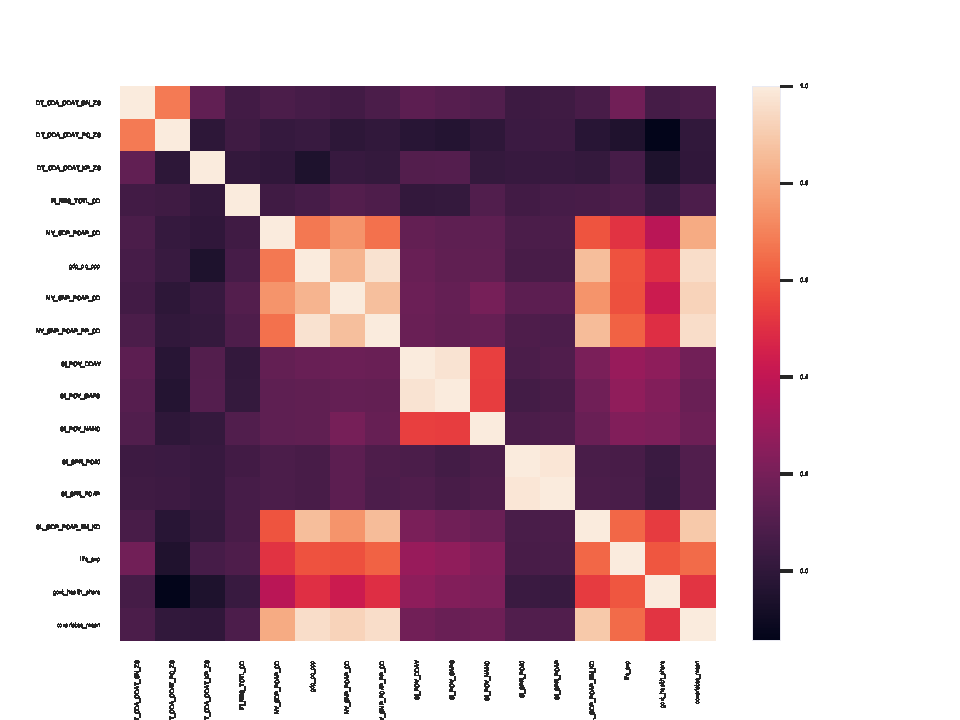
\includegraphics[width=\linewidth,keepaspectratio=true]{../Output/Figures/LE_Health_Econ_Correlations_wb_only_short.pdf}
        \end{figure}

        \begin{figure}[H]
            \centering
            \caption{Economic Measures PCA Loadings}
            \label{Econ_Loadings}	
            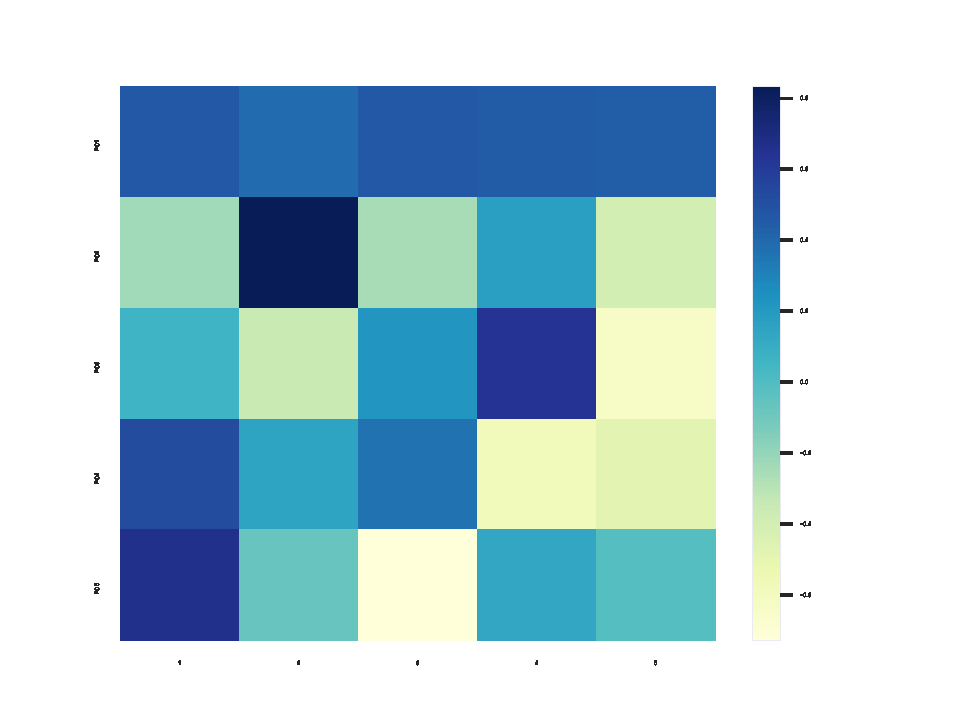
\includegraphics[width=\linewidth,keepaspectratio=true]{../Output/Figures/Econ_Indicator_Loadings_wb_only_short.pdf}
        \end{figure}

        \begin{figure}[H]
            \centering
            \caption{Economic Measures PCA Share of Variance Explained}
            \label{Econ_Share_Explained}	
            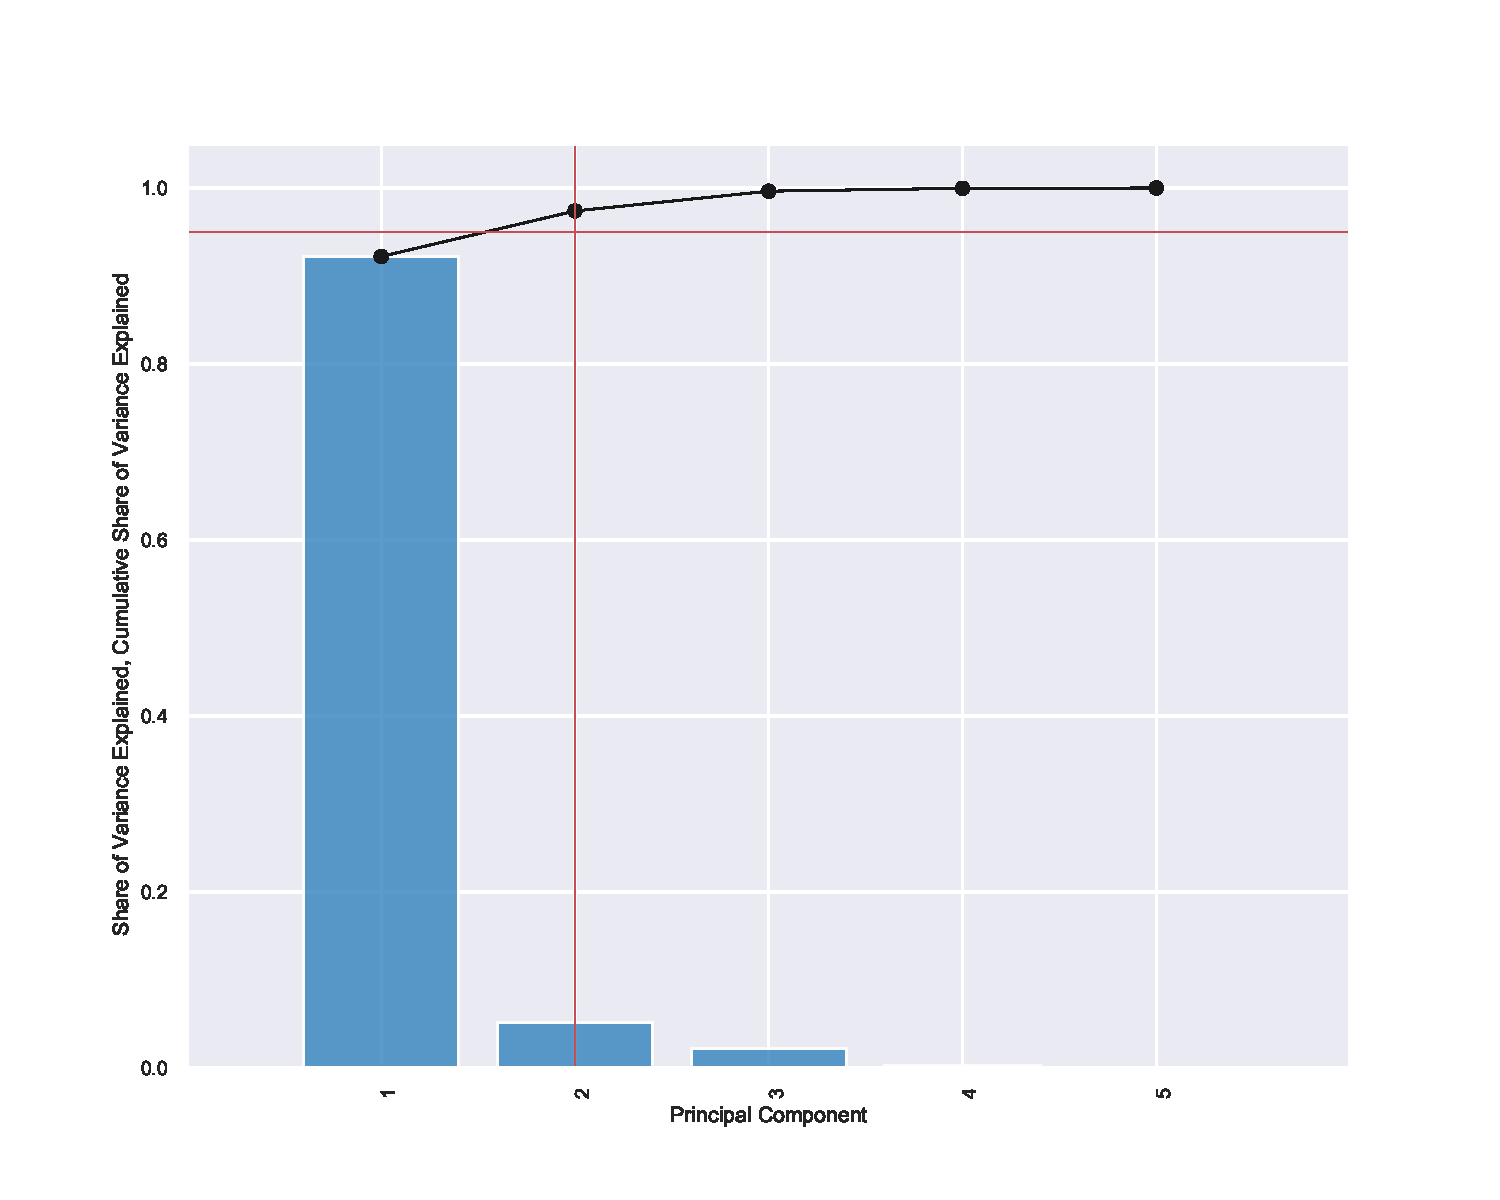
\includegraphics[width=\linewidth,keepaspectratio=true]{../Output/Figures/Econ_Indicator_Share_Explained_wb_only_short.pdf}
        \end{figure}

\end{document}